\documentclass{scrartcl}
\usepackage[T1]{fontenc}
\usepackage[utf8]{inputenc}
\usepackage[ngerman]{babel}
\usepackage{amsmath,amssymb}
\usepackage{graphicx}
\usepackage{enumerate}
\usepackage{calc}
\usepackage{ifthen}
\usepackage{multirow}
\usepackage{multicol}
\usepackage[left=2.0cm, right=2.0cm, top=2.0cm]{geometry}

\newcommand{\replicate}[2]{\ifnum#1>0 #2
	\expandafter\replicate\expandafter{\number\numexpr#1-1}{#2}\fi}

\renewcommand{\arraystretch}{1.5}

\newcounter{ctr} \setcounter{ctr}{1}

\setlength{\columnsep}{4cm}

\begin{document}	
\begin{multicols}{2}
{\Large O-Phasen-Gruppen:}\\[1em]
\begin{tabular}{|p{4cm}|p{1cm}|p{3cm}|}
\hline
\textbf{Gruppenname} & \textbf{Erstis} & \textbf{Aufteilung}\\ \hline
\replicate{26}{
 & & \\ \hline
}
\end{tabular}
\vfill\columnbreak

{\Large O-Lympia-Gruppen:}\\[1em]
\begin{tabular}{|c|p{5cm}|}
\hline
\textbf{Nr.} & \textbf{Gruppenname} \\ \hline
\replicate{13}{
A\arabic{ctr} & \\ \hline
B\arabic{ctr} & \stepcounter{ctr} \\ \hline
}
\end{tabular}
\end{multicols}
\clearpage
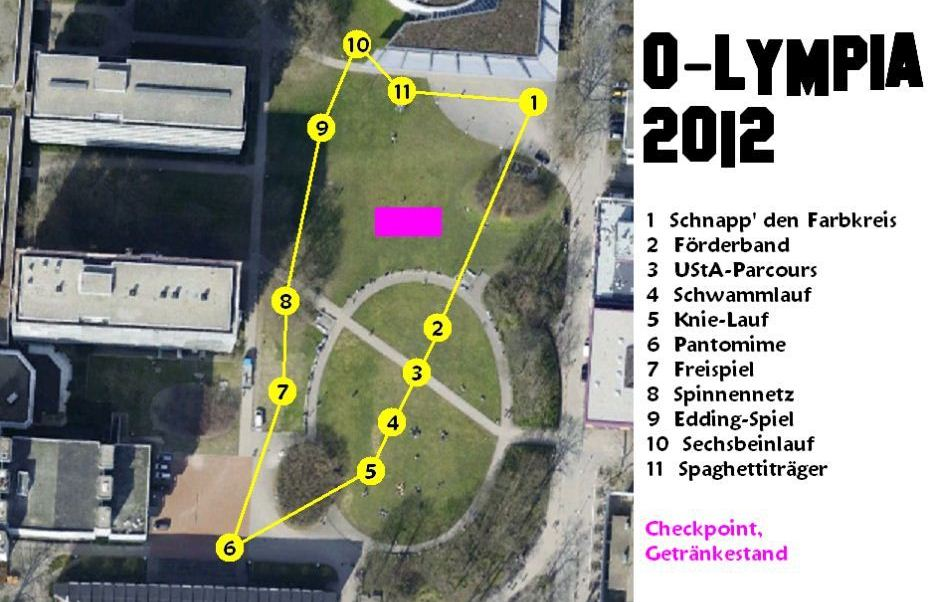
\includegraphics[scale=0.6]{spielplan_11.png}\\[2em]
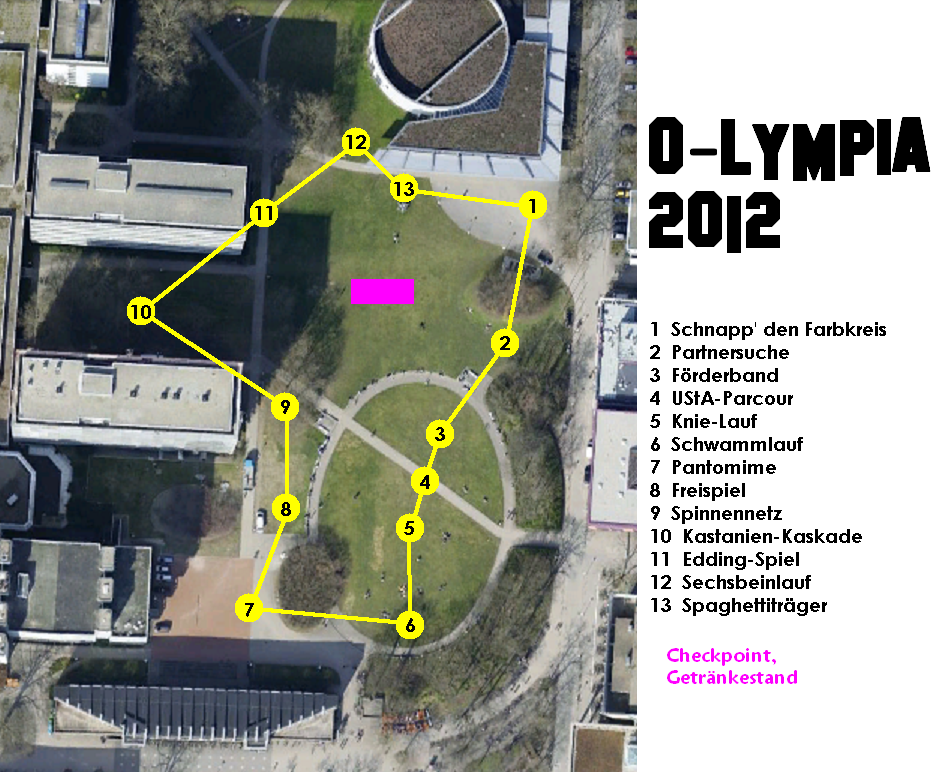
\includegraphics[scale=0.45]{spielplan.png}

\end{document}